\chapter{Prominence Observations}\label{Chap:obs}

\textit{The content of this chapter is based on work presented in sections 1, 2, and 3 of \cite{peat_solar_2021}.}

The prominence of 19 April 2018 observed with the Interface Region Imaging Spectrograph \citep[IRIS; ][]{depontieu_interface_2014} is the focus of this chapter. This observation has an IRIS OBSID of 3680113152.


\section{Configuration of the Observation}
\label{20180419main}
A filament appeared on the south western solar disc on 17 April 2018 in \ha\ observations from the Meudon Spectroheliograph\footnote{http://bass2000.obspm.fr} of the Observatoire de Paris (see Fig. \ref{ha}). 
\begin{figure*}
    \centering
    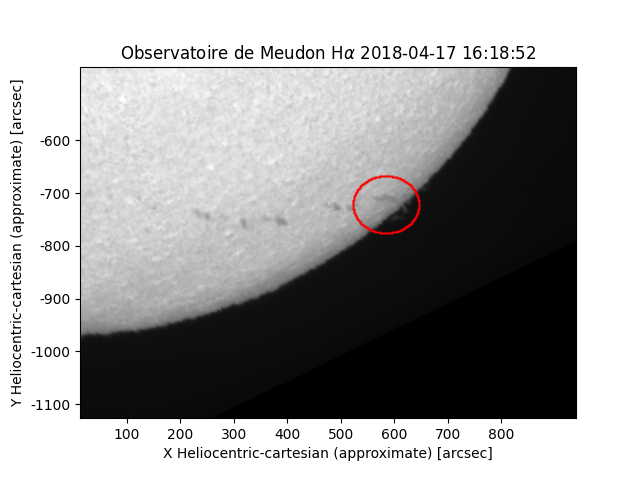
\includegraphics[width=0.8\linewidth]{./01Observations/figs/20180419/ha2.png}
    \caption[The prominence on the days leading up to the IRIS observations.]{The prominence (circled; appearing as a filament) on the days leading up to the IRIS observations. This plot is from \cite{peat_solar_2021}}
    \label{ha}
\end{figure*}
This later manifested as a prominence on the 19 April 2018 off the south western solar limb. This prominence was observed with IRIS, and Hinode \citep{kosugi_hinode_2007} as part of a coordinated observation with the Multichannel Subtractive Double Pass spectrograph \citep[MSDP; ][]{mein_solar_1991} in the Meudon Solar Tower, and the Atacama Large Millimeter/submillimeter Array \citep[ALMA; ][]{wootten_atacama_2009}. The IRIS and Hinode observations start at 14:14 and end at 19:15~UTC. The IRIS observations are made up of a set of 18 very large coarse 32-step rasters using the \ion{C}{ii} (1331.7~\AA-1358.3~\AA), \ion{Si}{iv} (1388~\AA-1406.7~\AA), and \mgii\ (2783.2~\AA-2835.0~\AA) filters along with their complementary slit-jaw imager (SJI) observations, centred on 1330~\AA, 1400~\AA, and 2796~\AA, respectively, with bandpasses of 55~\AA\ in the far-ultraviolet (FUV; \ion{C}{ii} and \ion{Si}{iv}), and 4~\AA\ in the near-ultraviolet (NUV; \mgii) SJI filters. The rasters had a field-of-view (FOV) of 63.9\arcsec$\times$182.3\arcsec\ centred on helioprojective coordinates 632.5\arcsec, $-$753.2\arcsec\ with a clockwise satellite rotation of 51\degr, so that the solar limb was approximately parallel to the y-axis of the instruments. The Hinode observations consisted of X-Ray Telescope \citep[XRT; ][]{golub_x-ray_2007} observations with the Al poly/Open, Open/Gband, and Open/Ti filter combinations with a FOV of 263.3\arcsec$\times$263.3\arcsec, centred on helioprojective coordinates of 607.2\arcsec, $-$749.7\arcsec. The MSDP observations start at 12:05 and end at 16:35~UTC, with a reconstructed FOV of 270\arcsec$\times$370\arcsec\ \citep{barczynski_spectro-imagery_2021}. The ALMA observations were undertaken in Band 3 (2.6-3.6~mm/84-116~GHz) from 15:20 to 17:45~UTC. The FOV of the ALMA observations are of an irregular shape, but are bounded by a box centred on 613.98\arcsec, -771.95\arcsec\ with sides of length 105.00\arcsec$\times$121.80\arcsec. This was the first high resolution interferometric observation of a solar prominence by ALMA \citep[see ][]{labrosse_first_2022}. Whole disc images from the Atmospheric Imaging Assembly \citep[AIA;][]{lemen_atmospheric_2012} onboard the Solar Dynamics Observatory \citep[SDO; ][]{pesnell_solar_2012} were also used. See Fig. \ref{config} for a schematic of this configuration.
  
\begin{figure}
    \centering
    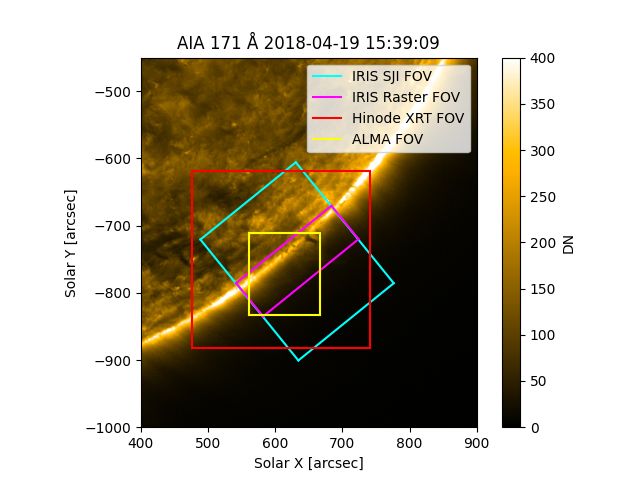
\includegraphics[width=0.93\linewidth]{./01Observations/figs/20180419/Figure_1.png}
    \caption[Configuration of instruments observing the prominence.]{Configuration of instruments observing the prominence. Please note, as the pointing of MSDP is not trivial to determine \citep{barczynski_spectro-imagery_2021}, it is not included in this plot. This plot is from \cite{peat_solar_2021}}
    \label{config}
\end{figure}
 
\begin{figure}
    \centering 
    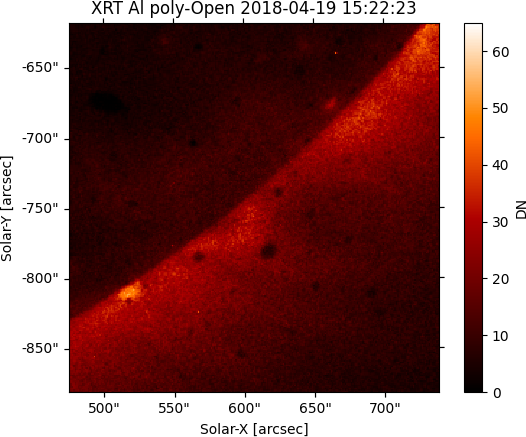
\includegraphics[width=0.6\linewidth]{./01Observations/figs/20180419/xrt.png}
    \caption[Hinode/XRT Al poly/Open observation of the prominence.]{Hinode/XRT Al poly/Open observation of the prominence. The coronal cavity can be clearly seen around (650\arcsec, $-$750\arcsec). This plot is from \cite{peat_solar_2021}}
    \label{xrt}
\end{figure}

The Open/Gband and Open/Ti XRT observations do not show anything of interest over the course of the observation. Al poly/Open also does not show any appreciable change or brightenings over the observation. However, the coronal cavity in which the prominence sits can be seen very clearly seen with this filter (see Fig. \ref{xrt}).

The main focus here is on the IRIS spectra and the information that can be gleaned from it. The IRIS FITS files were retrieved from the Lockheed Martin Solar and Astrophysics Laboratory (LMSAL) website\footnote{https://iris.lmsal.com/} as level 2 fits. Radiometric calibration was performed in Python using the method described in \cite{pereira_itn_2018}, with the appropriate response function retrieved from \texttt{https://hesperia.gsfc.nasa.gov/ssw/iris/response/} as described in \texttt{iris\_get\_response.pro} from SolarSoft \citep[SSW; ][]{freeland_data_1998}. It should be noted that IRIS is calibrated using data from the International Ultraviolet Explorer \citep[IUE;][]{bogges_IUE_1978}, and the spectral radiances recorded by this instrument are given an uncertainty of 10-15\%. As such, this introduces a similar uncertainty to the calibrated IRIS data \citep{tian_itn_2014}. The data was also deconvolved through Python following similar operations to that of \texttt{iris\_sg\_deconvolve.pro} from SSW\footnote{A full Python implementation of these procedures can be found at https://github.com/OfAaron3/irispreppy, or by simply running pip install irispreppy.}. The AIA files were retrieved from the Virtual Solar Observatory (VSO) as level 1 FITS. These were then prepared to level 1.5 through \texttt{aia\_prep.pro} from SSW in IDL. The 304~\AA\ filter shows similar behaviour to that seen in the \mgii~k SJI from IRIS. This is expected as both channels have high chromospheric to low transition region origins \citep{lemen_atmospheric_2012, depontieu_interface_2014}. 

The \mgii~k/2796~\AA\ SJI images show a very dynamic prominence with many flows, the bulk of which propagates towards the south-western limb \figp{threestages}. The observations culminate with a large flow extending down from the top of the prominence towards the southern solar limb.

The 171~\AA\ filter shows a small barb seen in absorption; this is where the prominence is anchored to the solar surface. This corresponds to the densest and most central part of the prominence. We expect to see strong central reversals in the area of the prominence due to the higher density in this location. In 171~\AA, we also see a faint shroud surrounding the barb, with its shape very similar to what is seen in 304~\AA. and \mgii~k. This can be interpreted as the prominence-to-corona transition region (PCTR) as the 171~\AA\ filter is senstive to spectral lines formed at transition region (TR) and coronal temperatures.

\begin{figure}
    \centering
    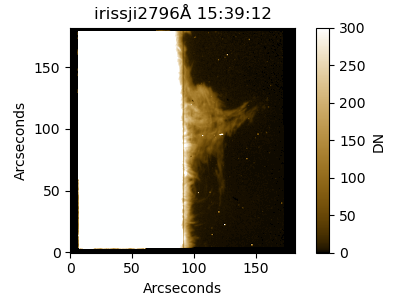
\includegraphics[width=0.32\linewidth]{./01Observations/figs/20180419/MgIISJI0.png}
    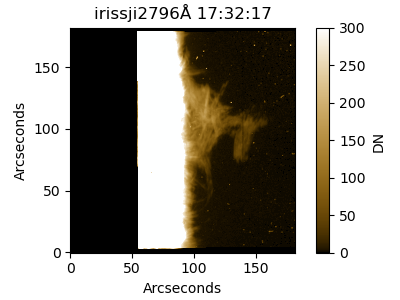
\includegraphics[width=0.32\linewidth]{./01Observations/figs/20180419/MgIISJI1.png}
    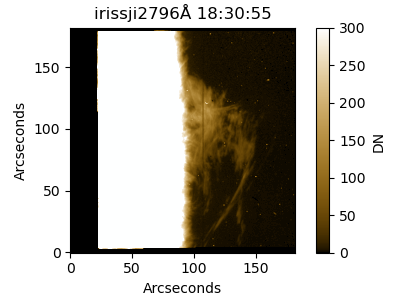
\includegraphics[width=0.32\linewidth]{./01Observations/figs/20180419/MgIISJI2.png}
    
    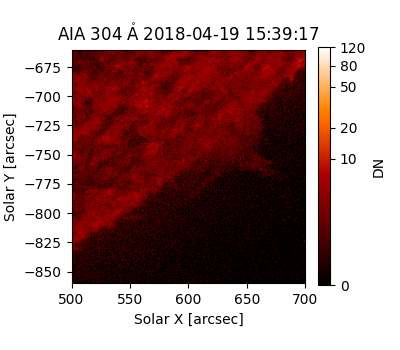
\includegraphics[width=0.32\linewidth]{./01Observations/figs/20180419/304_0.png}
    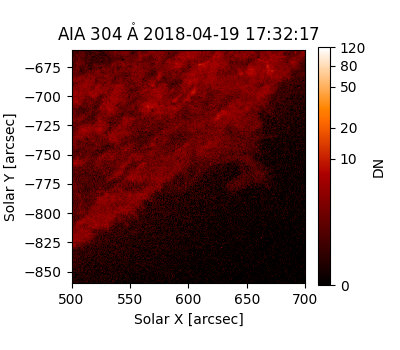
\includegraphics[width=0.32\linewidth]{./01Observations/figs/20180419/304_1.png}
    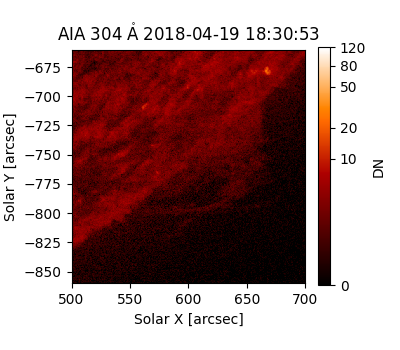
\includegraphics[width=0.32\linewidth]{./01Observations/figs/20180419/304_2.png}

    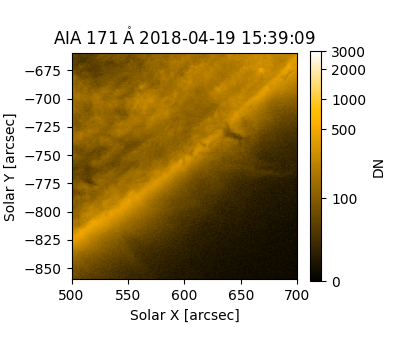
\includegraphics[width=0.32\linewidth]{./01Observations/figs/20180419/171_0.png}
    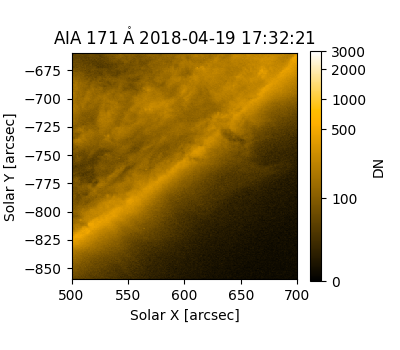
\includegraphics[width=0.32\linewidth]{./01Observations/figs/20180419/171_1.png}
    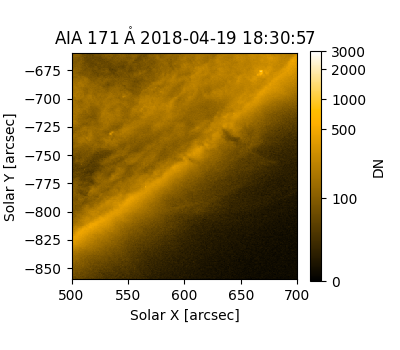
\includegraphics[width=0.32\linewidth]{./01Observations/figs/20180419/171_2.png}
    
    \caption[The key three stages of the development of the prominence.]{Observations of the prominence during the key three stages of its development. The top, middle, and bottom rows show the IRIS SJI \mgii~k, SDO/AIA 304\AA, and SDO/AIA 171\AA\ filters, respectively. \textit{Left} shows small flows towards the limb. \textit{Middle} shows the beginning of the large flow, where plasma extends out of the top of the prominence. \textit{Bottom} Shows the large flow towards the limb. These plots are from \cite{peat_solar_2021}.}
    \label{threestages}
\end{figure}

After the end of the IRIS, Hinode, MSDP, and ALMA observations, the prominence persists in 171~\AA{} and 304~\AA. In 304~\AA, the prominence continues to exhibit dynamic behaviour and appears to fall towards the limb over the next 24 hours. This is a consequence of the projection effect, as it rotates out of view. This behaviour is not mirrored in 171~\AA. The barb and shroud instead appear to fade away as they become occulted by brighter coronal emission. On 22 April, the structure appears again in the 171~\AA{} and 304~\AA{} filters of EUVI, part of the Sun Earth Connection Coronal and Heliospheric Investigation \citep[SECCHI; ][]{howard_sun_2008} on board the Solar Terrestrial Relations Observatory (Ahead) \citep[See Fig \ref{secchi}; STEREO-A; ][]{driesman_stereo_2008}. The prominence is observed to continue to transit across the disc and no filament eruption is observed. At this time, STEREO-A was approximately 117\degr{} west of the Earth.

\begin{figure}
    \centering
    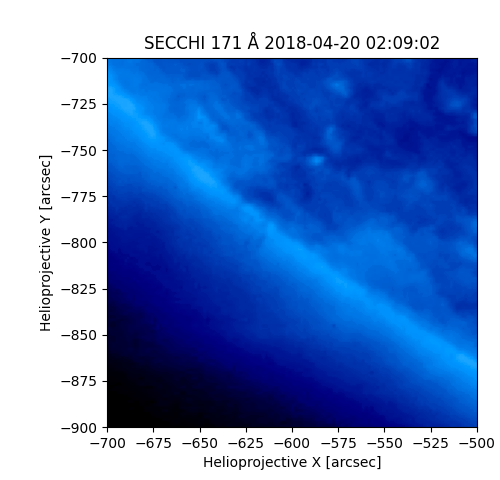
\includegraphics[width=0.49\linewidth]{./01Observations/figs/20180419/secchi171.png}
    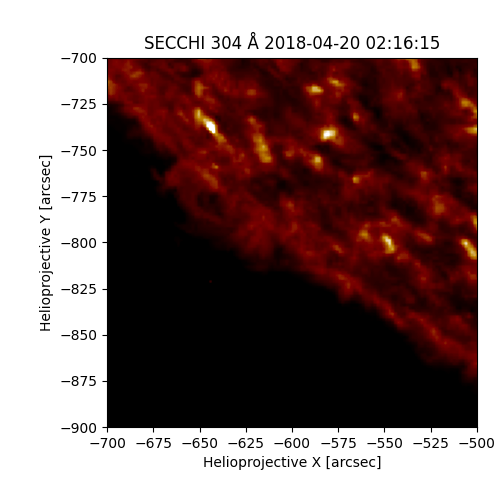
\includegraphics[width=0.49\linewidth]{./01Observations/figs/20180419/secchi304.png}
    \caption[The prominence as it appears on the 20 April 2018 in EUVI on SECCHI.]{The prominence as it appears on the 20 April 2018 in EUVI on SECCHI. \textit{Left}: The prominence barb reappearing in 171~\AA. \textit{Right}: The prominence structure in 304~\AA.}
    \label{secchi}
\end{figure}

\begin{figure}
    \centering
    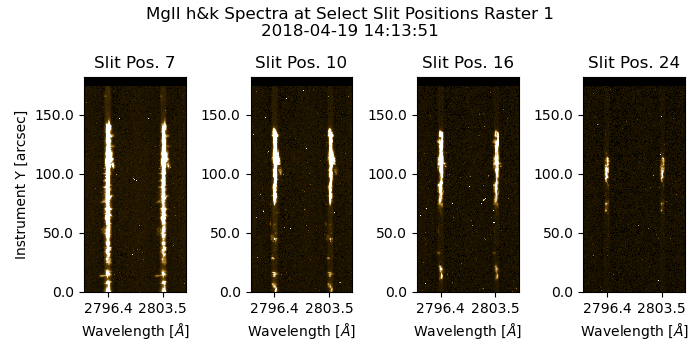
\includegraphics[width=.85\linewidth]{./01Observations/figs/20180419/slit1.png}
    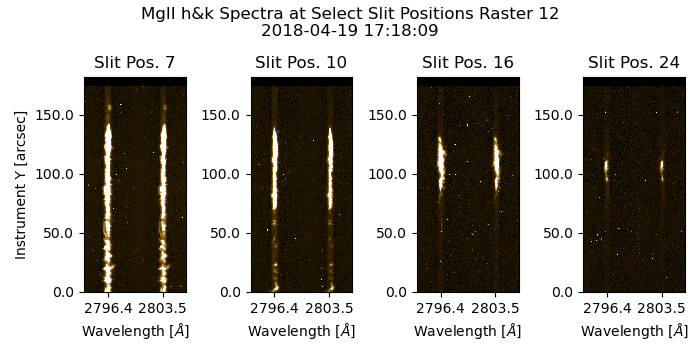
\includegraphics[width=.85\linewidth]{./01Observations/figs/20180419/slit12.png}
    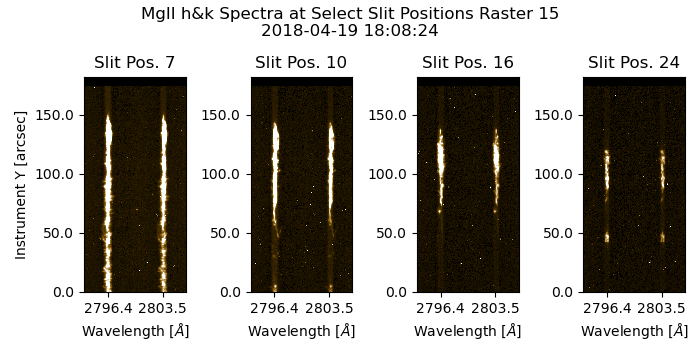
\includegraphics[width=.85\linewidth]{./01Observations/figs/20180419/slit15.png}
    \caption[\mgiihk\ at select slit positions and rasters. See Fig. \ref{fig:hmaps} and Fig. \ref{fig:kmaps} for context.]{\mgiihk\ at select slit positions and rasters. See Fig. \ref{fig:hmaps} and Fig. \ref{fig:kmaps} for these slit position in context. There is a wide range of profile shapes present, and a few where several structures are clearly present. These plots are from \cite{peat_solar_2021}.}
    \label{spectra}
\end{figure}

\begin{figure}
    \centering
    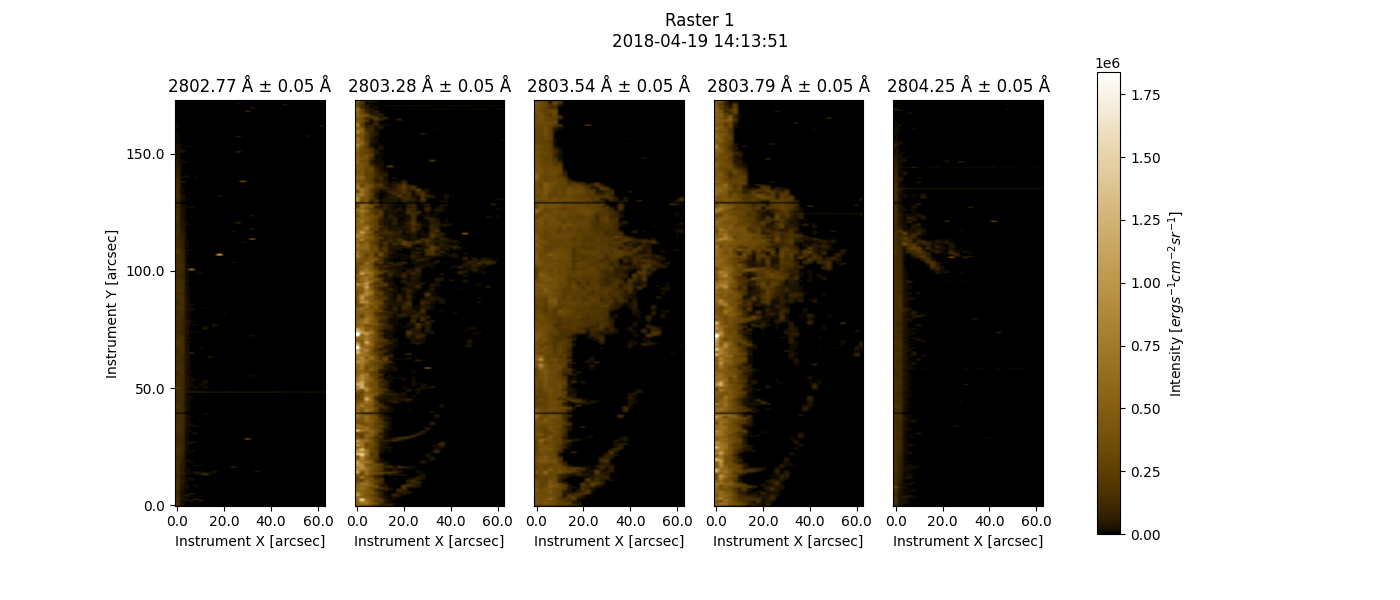
\includegraphics[width=0.9\linewidth]{01Observations/figs/20180419/spectrogramh1.png}
    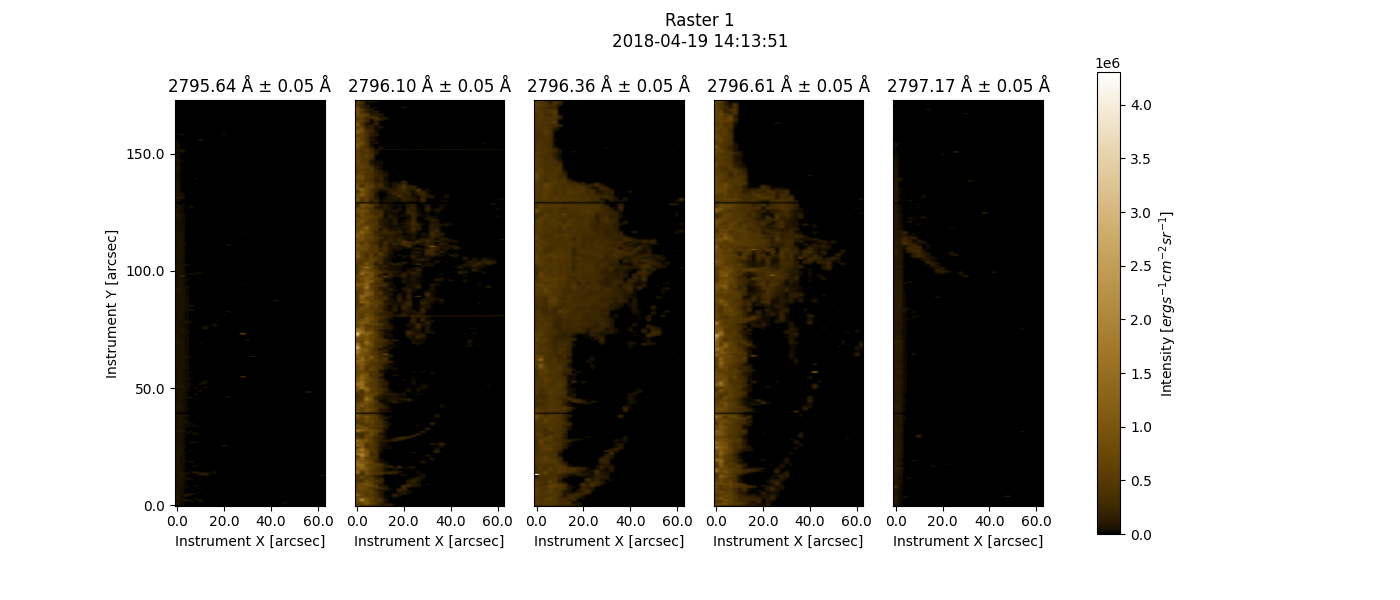
\includegraphics[width=0.9\linewidth]{01Observations/figs/20180419/spectrogramk1.png}
    \caption[\mgiihk{} maps at different points along the wavelength window. In the rightmost/redshift panel, an isolated structure is observed.]{\mgiihk\ (top and bottom respectively) maps at different points along the wavelength window. In the rightmost/redshifted panel, an isolated structure is observed.}
    \label{fig:extraboi}
    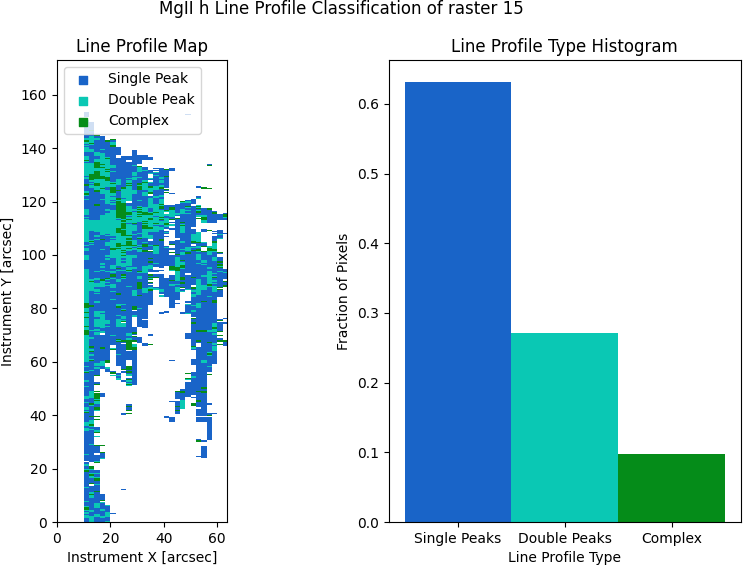
\includegraphics[width=.47\linewidth]{./01Observations/figs/20180419/h14lt.png}
    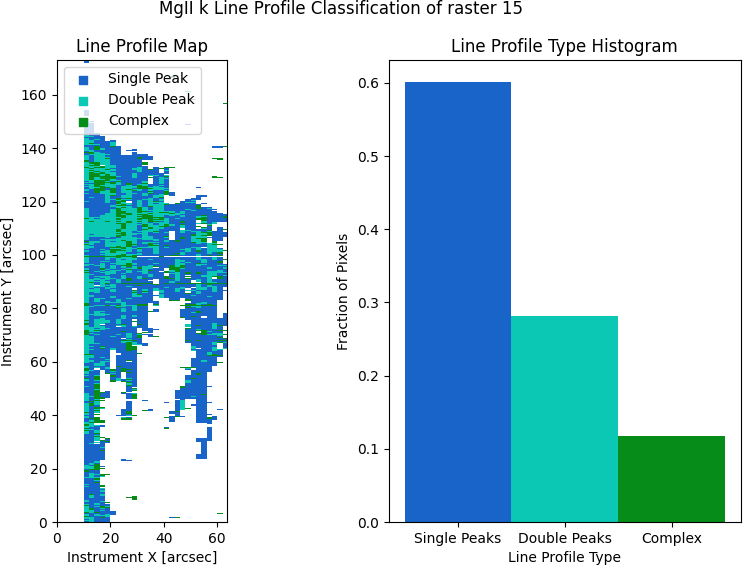
\includegraphics[width=.47\linewidth]{./01Observations/figs/20180419/k14lt.png}
    \caption[Distribution of line types seen in \mgiihk\ in raster 14.]{Distribution of line types seen in \mgiihk\ in raster 14. A complex line profile is any line profile found to have two or more than three turning points. The left plot is from \cite{peat_solar_2021}}
    \label{linetypes}
\end{figure}

\begin{figure} 
    \centering
    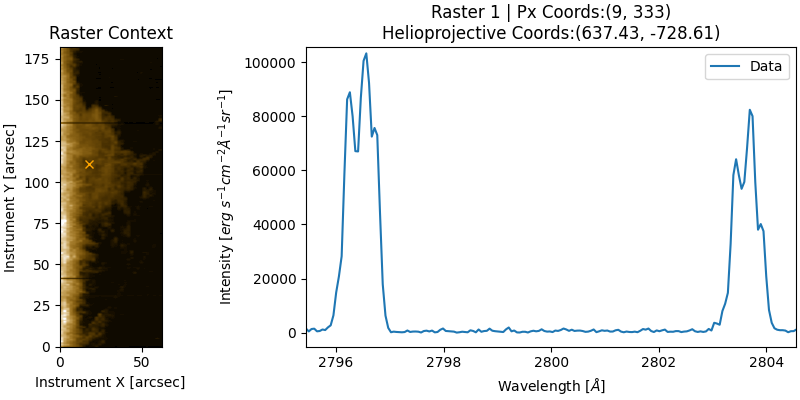
\includegraphics[width=0.8\linewidth]{./01Observations/figs/complex.png}
    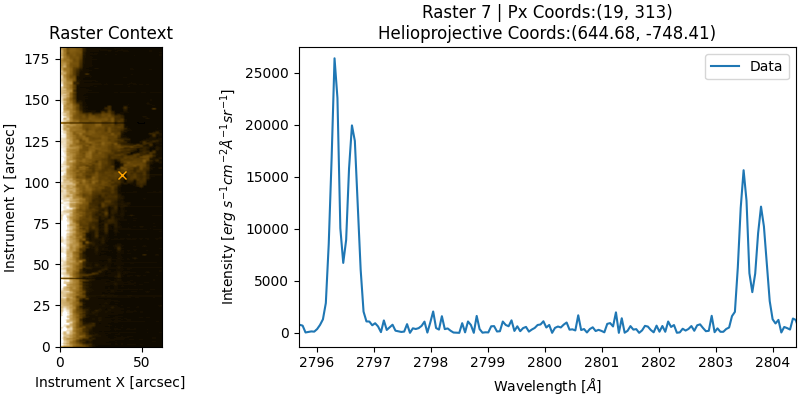
\includegraphics[width=0.8\linewidth]{./01Observations/figs/double.png}
    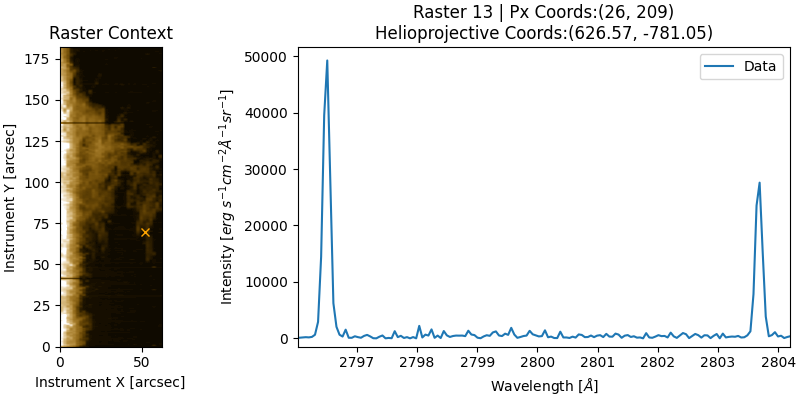
\includegraphics[width=0.8\linewidth]{./01Observations/figs/single.png}
    \caption{Examples of the three different classifications of peaks. \textit{Top}: Complex. \textit{Centre}: Double peaked. \textit{Bottom}: Single peaked.}
    \label{threespectratypes}
\end{figure}

The \mgii~h\&k spectra from the core of the prominence display many complex structures. This carries the implication that there are many structures along the line of sight. One notable example of this can be seen in the top panel of Fig. \ref{spectra} at approximately 110\arcsec\ in slit position 7. Here there are clearly two different peaks, one near the rest wavelength, and a second highly redshifted. This can be seen more clearly in \fig{fig:extraboi}. The structure producing these highly redshifted peaks is very easily seen through the wings of the at-rest \mgii\ in front of it. This structure is likely behind the prominence as it disappears in the subsequent rasters. This occurrence is not unique to this case, and is quite common throughout the prominence. This is, however, the most extreme example. As one may expect, the prominence  spectra are composed of many different types of line profiles. This distribution can be seen in Fig. \ref{linetypes}. To find the distribution of line profile types, the numerator of the difference quotient was solved for each pixel in a 3~\AA{} window centred on \mgiihk{}, respectively,
\begin{equation}
    \frac{df(\lambda)}{d\lambda}=\frac{f(\lambda+\Delta\lambda)-f(\lambda)}{\Delta\lambda}.
\end{equation}
If the numerator changed polarity between two successive pixels, this was counted as a turning point. If one turning point was found, that pixel would be classed as having a single peak; if three were found, it would be classed as a reversed profile; if any other number was found, it would be classed as complex. The classification of any line profile with two peaks is ambiguous, and so is classed as complex (see \fig{threespectratypes} for an example of these). To avoid counting turning points in the noise, an intensity threshold was set, where any turning point below that intensity threshold was discarded.While single peak profiles dominate the distribution, double peaked and complex profiles are not negligible, with roughly 10\% to 20\% of the profiles appearing complex in both h and k. The large branch observed to be extending towards the limb near the end of the observation appears to exhibit mostly single peaked profiles along with some double peaks. Additionally, it appears to have some profiles classed as single peaks that are in fact double peaks suffering from an effect further discussed in Sect. \ref{velsect}, where the emission of h$_{2r}$ and k$_{2r}$ is lower than that of h$_{3}$ and k$_{3}$, therefore no turning point is produced here. This results in only the h$_{2v}$ and k$_{2v}$ peaks being pronounced enough such that $\dd I/\dd \lambda=0$ at these peaks. This effect is also present in the reverse scenario. This can be interpreted in one of two ways - the line profile is double peaked, but is so Doppler shifted that one of the peaks ends up in the rest line core and is absorbed; or there exists more than one thread of plasma at different line-of-sight velocities leading to a false double peak. In the former case, the plasma would require high density, temperature or large geometrical thickness to produce a double peak, and then it would require a large line-of-sight velocity to produce this effect. The latter, however, has less extreme prerequisites. Additionally, prominences are known to be comprised of many threads moving at a plethora of line-of-sight velocities \citep{engvold_fine_1978}, and so we interpret this as such \seef{k2vgtk2r}.

\begin{figure} 
    \centering
    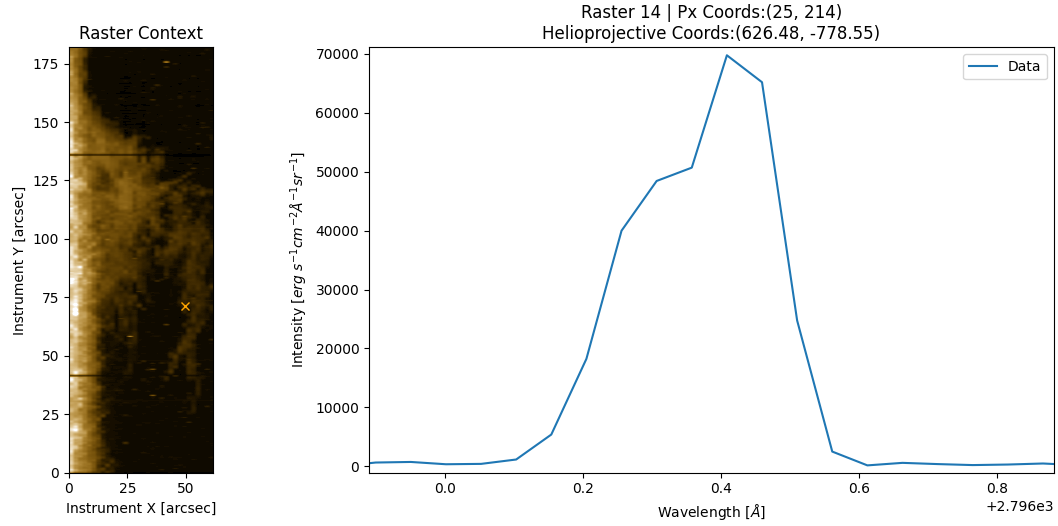
\includegraphics[width=0.7\linewidth]{./01Observations/figs/asym.png}
    \caption{Asymmetry in \mgii~k where it could be argued that there are two peaks due to there likely being two threads along the line of sight. However, this profile was classified as having a single peak.}
    \label{k2vgtk2r}
\end{figure}






% \begin{figure}
%     \centering

% \end{figure}
Here, we focus mainly on the NUV filter of IRIS. The prominence appears only very faintly in the FUV bands, making analysis difficult. Additionally, increasing the contrast in the FUV bands enough to see the prominence leads to the appearance of a ghost image of the aperture of the telescope on the image. This is due to parasitic light and only affects FUV off-limb observations, the NUV channels are unaffected by this \citep{wulser_instrument_2018}.
\section{The Quantile Method}
\label{quantile_method}
\begin{figure}
    \centering
    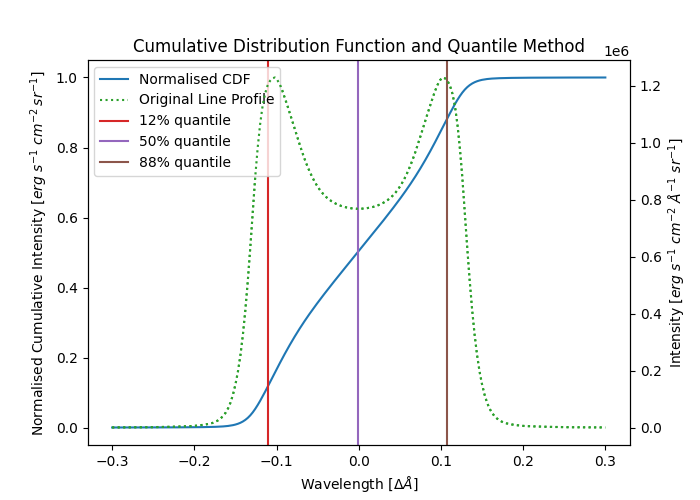
\includegraphics[width=.9\linewidth]{./01Observations/figs/20180419/cdf.png}
    \caption{Cumulative Distribution Function of a synthetic line profile as an example; with its associated 12\%, 50\%, and 88\% quantiles.}
    \label{cdfex}
\end{figure}

We use the quantile method \citep{kerr_iris_2015,ruan_dynamic_2018} to determine the FWHM, line core shift, and asymmetry of the line profiles to explore the dynamics and structure of the prominence. The quantile method involves calculating the cumulative distribution function (CDF) over the intensity of the line profiles over some wavelength range. We use two 3~\AA\ windows centred on the rest wavelengths of \mgiihk. We then linearly interpolate over these CDFs to find the wavelengths corresponding to the 12\%, 50\%, and 88\% levels of the CDFs ($\lambda_{12}, \lambda_{50}, \lambda_{88}$). $\lambda_{50}$ is defined as the line core and is used to find the line core shift in km~s$^{-1}$. To obtain a value for $\lambda_\text{rest}$, we applied the quantile method on the first slit of the raster. This first slit is on the solar disc, and we employ a 3\AA{} window centred on the rest vaccuum wavelengths of \mgiihk{}, respectively, to obtain a value for the rest wavelengths of both h and k. The mean of these rest wavelengths, in h and k, was then taken and used as $\lambda_\text{rest}$ in \eq{eq:vdop}. Assuming that the lines are Gaussian in nature, the FWHM can be determined by finding the difference between $\lambda_{88}$ and $\lambda_{12}$. However, not all of our profiles are Gaussian, and we instead use this as a measurement of line width. All three of these values are used to determine the asymmetry. As equations, they are as follows,

\begin{equation}
    v_\text{dop}=\left(\frac{\lambda_{50}}{\lambda_{\text{rest}}}-1\right)c,
    \label{eq:vdop}
\end{equation}
\begin{equation}
    \text{Line Width}=~\lambda_{88}-\lambda_{12},
    \label{eq:fwhm}
\end{equation}
\begin{equation}
    \text{Asymmetry}=~\frac{\left(\lambda_{88}-\lambda_{50}\right)-\left(\lambda_{50}-\lambda_{12}\right)}{\lambda_{88}-\lambda_{12}},
    \label{eq:asym}
\end{equation}
%overfull hbox craziness be here. This comment fixes it.
where $\lambda_{\text{rest}}$ is the rest wavelength of the line, and $c$ is the speed of light. A graphical representation of these quantiles can be seen in Fig. \ref{cdfex}. The maps resulting from these equations can be seen in Figs. \ref{fig:hmaps} and \ref{fig:kmaps} for h\&k, respectively.
 
Coronal pixels were removed from the \mgii~h\&k rasters using the quantile method. From line width maps, chromospheric-like structures, such as the prominence and spicules, are very clearly separated from the solar disc and coronal pixels \sectp{lwid}. Therefore, by calculating the line width of every pixel for every raster via the quantile method coronal pixels could be removed. Coronal pixels will be found to exhibit large line widths compared to data and will be clearly separated in a histogram. This is not a true measure of line width, as in coronal pixels there is no \mgiihk{} emission to measure here, but the method still returns a value. This produces a double peaked distribution in the line width histogram. The minimum turning point of this distribution is selected as the cut off value, where values higher than this are considered to be coronal pixels \figp{lwHist}. However, some non-coronal pixels truly do have a large line width. To combat these false positives, the pixels are then subject to a simple intensity filter. Any of these would-be discarded pixels that are above the threshold are relabelled as not coronal. This limit was set as twice the mean intensity of every pixel of every raster in two 3~\AA\ wide windows centred on the rest wavelengths of \mgiihk, respectively.  The result of this filtering can be seen in Fig. \ref{filtresult}. Since the publication of \cite{peat_solar_2021}, the work on which this section is based, this filter now includes an extra step to remove any rogue coronal pixels that slip through the filter. Inspired by the death by underpopulation rule from John Conway's Game of Life \citep{martin_mathematical_1970}, any unremoved pixel that has 2 or fewer unremoved 2-connected neighbours (the surrounding pixels) is also removed. 

In order to estimate the error associated with the Doppler velocity, line width and asymmetry, a synthetic double peaked line profile was used from PROM \sectp{promintro}. This profile was downscaled to the same resolution as the IRIS spectrograph and padded with zeros such that it was 3~\AA{} wide. Then, using the filtered rasters, the every pixel's mean value between 2797.85~\AA{} and 2802.03~\AA{} was taken. The standard deviation and mean of these values were taken in order to estimate Gaussian noise. This noise was randomly added to the synthetic line profile and the Doppler velocity, line width, and asymmetry were calculated using the quantile method for \mgiihk, respectively. This was repeated one million times to acquire a large sample size. A Gaussian was then fitted to the histograms of these distributions in order to recover a standard deviation which we will quote as the error of these measurements. For \mgii~h, the standard deviations were found to be $0.369$~\kms, $3.94\times10^{-3}$~\AA, and $2.00\times10^{-2}$~\AA{} for Doppler velocity, line width, and asymmetry, respectively. For \mgii~k, the standard deviations were found to be $0.225$~\kms, $2.03\times10^{-3}$~\AA, and $1.58\times10^{-2}$~\AA{} for Doppler velocity, line width, and asymmetry, respectively.

\begin{figure}
    \centering
    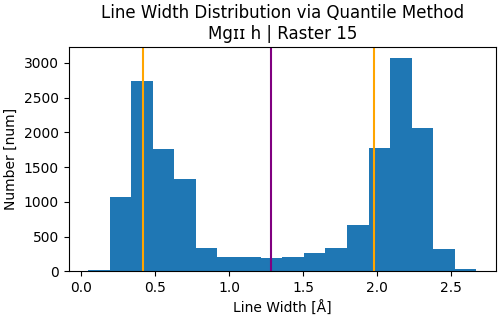
\includegraphics[width=0.49\linewidth]{./01Observations/figs/h15.png}
    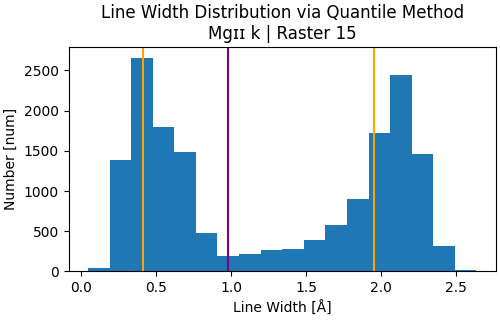
\includegraphics[width=0.49\linewidth]{./01Observations/figs/k15.png}
    \caption[Histogram of the line widths of \mgiihk{} in raster 15.]{Histogram of the line widths of \mgiihk{} in raster 15. The purple vertical line indicates the local minimum and cut off point and the orange lines represent the range over which the minimum turning point is searched for.}
    \label{lwHist}
\end{figure}

\begin{figure}
    \centering
    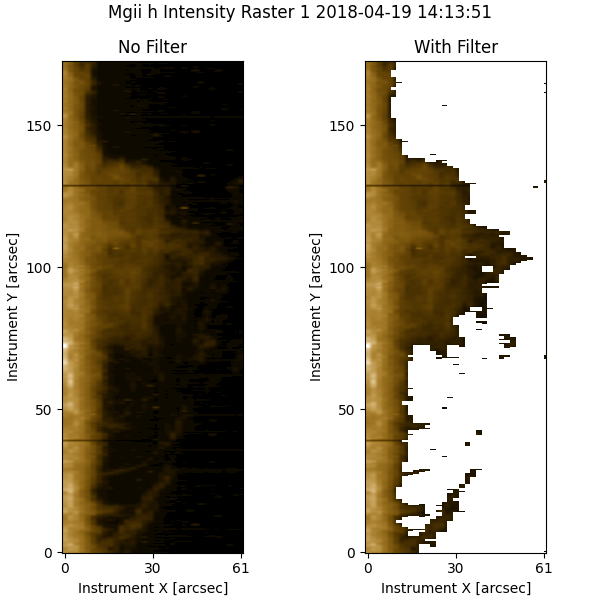
\includegraphics[width=0.6\linewidth]{./01Observations/figs/20180419/Figure_2.png}
    \caption[Example of a resulting \mgii~h map with the filtering applied.]{Example of a resulting \mgii~h map with the filtering applied. \textit{Left}: \mgii~h without the filter and \textit{Right}: \mgii~h with the filter. This plot is from \cite{peat_solar_2021}}
    \label{filtresult}
\end{figure}



\begin{figure}
    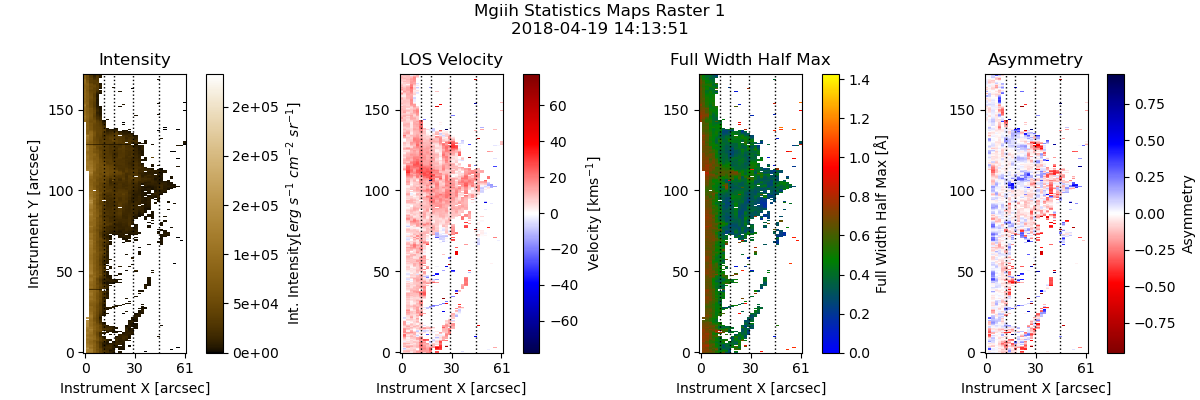
\includegraphics[width=\linewidth]{./01Observations/figs/20180419/hmaps0.png}
    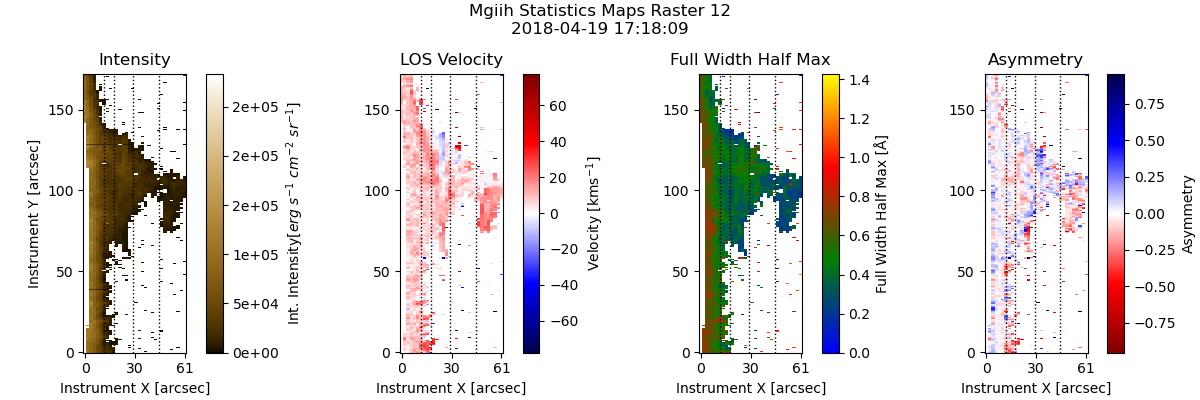
\includegraphics[width=\linewidth]{./01Observations/figs/20180419/hmaps1.png}
    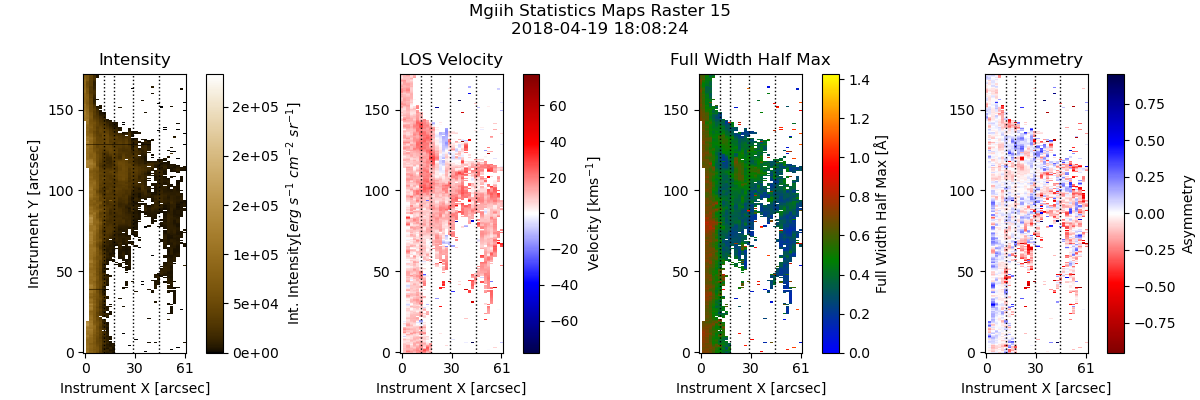
\includegraphics[width=\linewidth]{./01Observations/figs/20180419/hmaps2.png}
    \caption[\mgii~h statistics maps of the three main stages of the prominence.]{\mgii~h statistics maps of the three main stages of the prominence observation calculated via equations \ref{eq:vdop}, \ref{eq:fwhm}, and \ref{eq:asym}. The times associated with these plots are the time at the beginning of the associated raster scan. The four dotted lines correspond to the spectra presented in Fig. \ref{spectra}. These plots are from \cite{peat_solar_2021}.}
    \label{fig:hmaps}
\end{figure}

\begin{figure}
    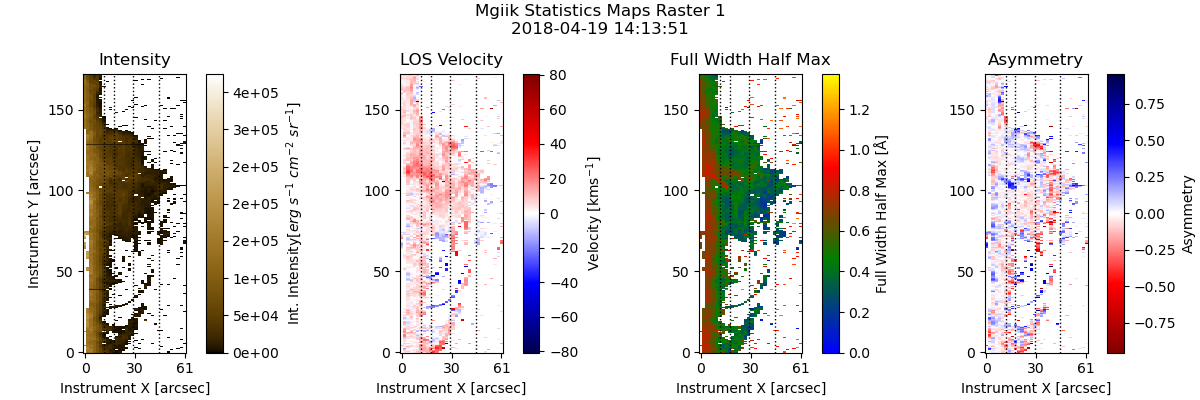
\includegraphics[width=\linewidth]{./01Observations/figs/20180419/kmaps0.png}
    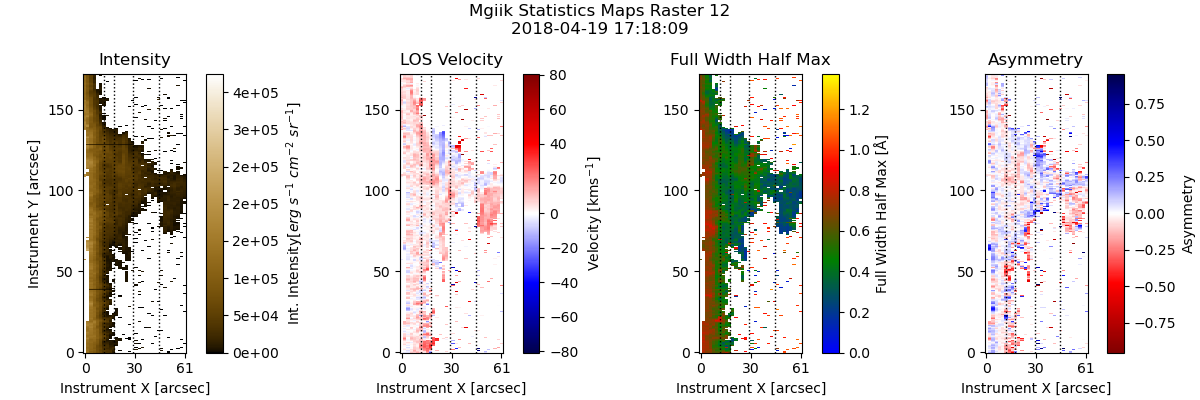
\includegraphics[width=\linewidth]{./01Observations/figs/20180419/kmaps1.png}
    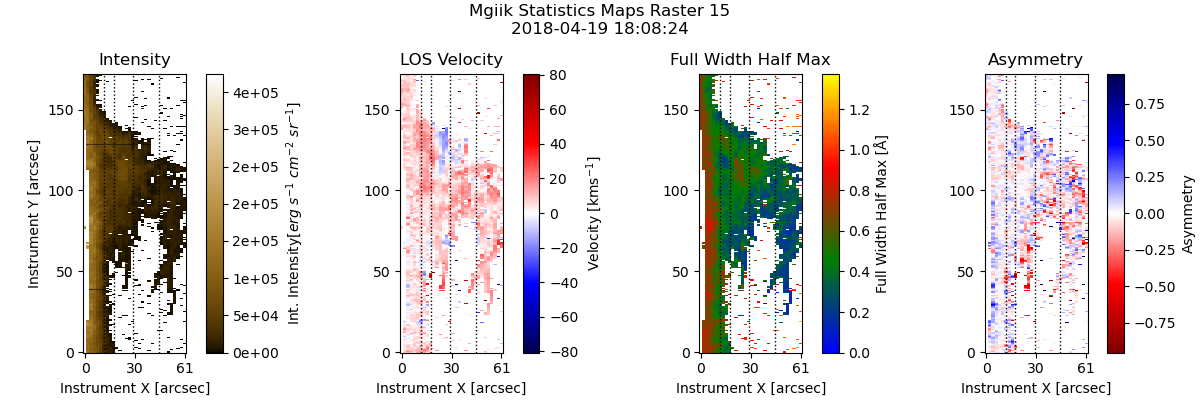
\includegraphics[width=\linewidth]{./01Observations/figs/20180419/kmaps2.png}
    \caption[\mgii~k statistics maps of the three main stages of the prominence.]{Same as \fig{fig:hmaps} for \mgii{}k. This plot is from \cite{peat_solar_2021}.}
    \label{fig:kmaps}
\end{figure}

\section{Line Core Shift and Asymmetry}
\label{velsect}

The prominence displays a wide range of line core shift ranging from $-$74 to 78~km~s$^{-1}$ and $-$72 to 85~km~s$^{-1}$ in \mgiihk, respectively. Both display Gaussian-like distributions centred on a mean redshift of 8.20~km~s$^{-1}$ and 5.2~km~s$^{-1}$ with standard deviations of 5.98~km~s$^{-1}$ and 6.61~km~s$^{-1}$, respectively. The extreme velocities found here are very rare, and this is reflected in \fig{fig:velgauss} where most material is found to be moving in the range -20\kms{} to 30\kms.  
\begin{figure}
    \centering
    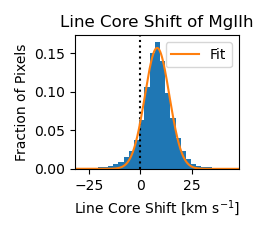
\includegraphics[width=0.35\linewidth]{./02Modelling1D/figs/20180419/hvelocities.png}
    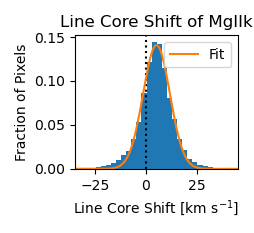
\includegraphics[width=0.35\linewidth]{./02Modelling1D/figs/20180419/kvelocities.png}
    \caption[Distribution of line core shifts found in the prominence.]{Distribution of line core shifts found in the prominence. \textit{Left}: \mgii~h. \textit{Right}: \mgii~k. These plots are from \cite{peat_solar_2021}.}
    \label{fig:velgauss}
\end{figure}
These velocities are consistent with those seen in past observations. \cite{liggett_rotation_1984} observed velocities ranging from 12 to 75~km~s$^{-1}$; \cite{schmieder_reconstruction_2017} found maximum velocities of around 60~km~s$^{-1}$; and Table 6 from the review by \cite{labrosse_physics_2010} shows a range of velocities exhibited by EUV prominences with an extreme of 70~km~s$^{-1}$, centred around 20\kms. The Gaussian fits used to model the distributions of line core shifts does not seem to match well at the wings. This may be due to ``asymmetry bias'', where line profiles with large asymmetry are mistakenly measured to have a large Doppler velocity via the quantile method. This is due to the increased influence of h$_{2\text{v}}$/k$_{2\text{v}}$ for those of high blueshift, or h$_{2\text{r}}$/k$_{2\text{r}}$ for those with high redshift, as these peaks move into the more optically thin regime in the wings, increasing their peak intensity. This effect is further exaggerated by the opposite effect, where the h$_{2\text{r}}$/k$_{2\text{r}}$ for high blueshift, or the h$_{2\text{v}}$/k$_{2\text{v}}$ for high redshift, move into the more optically thick regime in the core, decreasing their peak intensity. This is not something that can be simply corrected for if we wish to continue using the quantile method. This effect is illustrated in Fig. \ref{fig:hda}. It is then therefore suggested that the line core shift found by the quantile method in areas of high asymmetry are not to be trusted. Line core shifts of pixels are therefore more reliable the closer to zero their respective asymmetry. Line core shift and asymmetry are very strongly linked. Line profile asymmetry is strongest in the branch extending down from the main body near to the end of the rasters. The asymmetries of these line profiles are in the range [0, -1), suggesting, as discussed in Sect. \ref{velsect}, that many of these may be highly redshifted. This is true, but the branch is mainly comprised of single profiles which are not so sensitive to this effect. Instead we observe a mix of asymmetrical line profiles, and low intensity and low width lines \figp{asyms}. Our wide 3~\AA\ window causes the quantile method to measure overestimate the asymmetry of the latter. This could be another explanation for the relationship seen in \fig{fig:hda}. Asymmetry and line core shift appear to be anticorrelated as shown in \fig{fig:hda}, however, the structure around 110~\arcsec in raster 1 appears to break this trend. Therefore, the asymmetry and line width, calculated via the quantile method, together would perhaps be a better proxy for whether a pixel contains more than one profile, rather than line width alone. This may be the reason that we observe an overall redshift from even though we have corrected for solar rotation. 

It is difficult to quantify the uncertainty that the asymmetry causes on the measurement of line core shift. This is because you are required to know the `true' line core shift. This is not easily determined due to the multithreaded nature we see in line profiles from solar prominences. By that rationale, one could argue that the measurements of line core shift themselves are not entirely reliable either. This brings us back to the same conclusion from earlier where we suggest that line core shifts of pixels are more reliable the closer to zero their respective asymmetry.

\begin{figure}
    \centering
    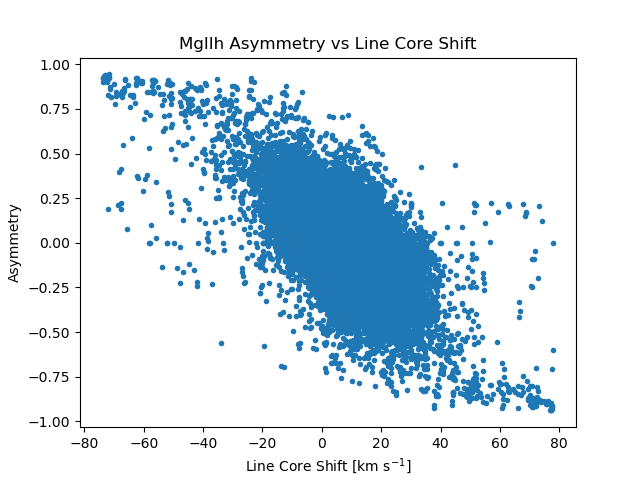
\includegraphics[width=0.7994\linewidth]{01Observations/figs/20180419/hda.png}
    \caption[Asymmetry against line core shift for all prominence pixels in every raster.]{Asymmetry against line core shift for all prominence pixels in every raster. This demonstrates the effect of ``asymmetry bias'' when measuring line core shift with the quantile method. This plot is from \cite{peat_solar_2021}}
    \label{fig:hda}
\end{figure}

\section{Line Widths}
\label{lwid}
As mentioned in Sect. \ref{quantile_method}, line width is measured by \eq{eq:fwhm}. The line width maps clearly separate the chromospheric-like structures, such as the prominence and spicules, from the solar disc, with the disc displaying line widths of greater than approximately 0.8~\AA\ and the spicules and the prominence displaying much less. As discussed in Sect. \ref{20180419main}, it also clearly distinguishes the coronal pixels from the prominence. This of course, is not shown on the Fig. \ref{fig:hmaps} and Fig. \ref{fig:kmaps} as it is filtered out. The large measured line width is just a consequence of using the quantile method to measure the line widths. There are no \mgiihk\ line profiles in the corona to measure the width of, but a CDF is still created and analysed as if there were \mgiihk{} emission. In non-filtered diagnostic maps, line width is a good way to view the bulk motion of low intensity features difficult to distinguish in intensity maps \figp{fwhmex}.

\begin{figure}
    \centering
    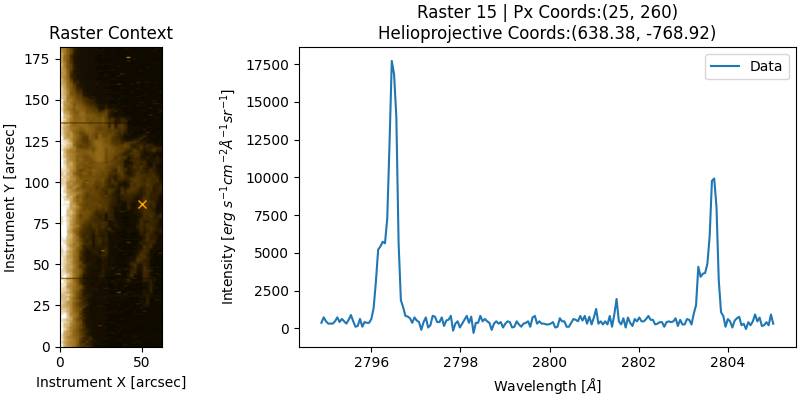
\includegraphics[width=0.6\linewidth]{./01Observations/figs/20180419/asym1.png} 
    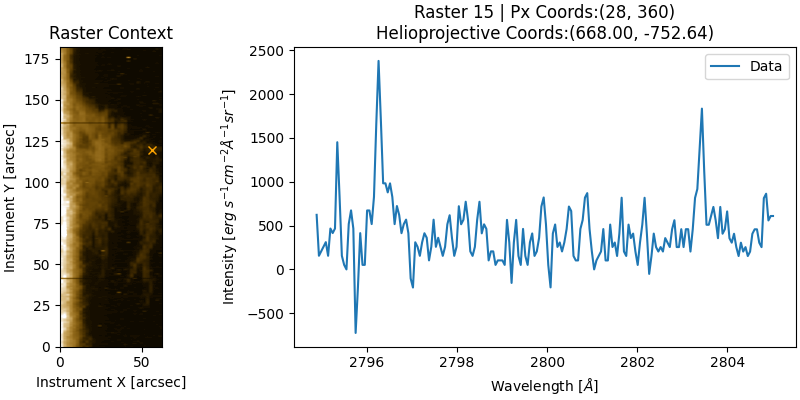
\includegraphics[width=0.6\linewidth]{./01Observations/figs/20180419/asym4.png}
    \caption[Two examples of the types of \mgiihk{} line profiles seen in the branch]{Two examples of the types of \mgiihk{} line profiles seen in the branch. \textit{Top}: Asymmetric line profiles. \textit{Bottom}: Low intensity and line width lines.}
    \label{asyms}
\end{figure}


In the first raster (14:13:51~UTC), we see a structure of large line width around 110\arcsec\ in y. This is due to the presence of at least two structures along the line of sight, with one highly redshifted profile. This can be seen in Fig. \ref{fig:extraboi}, where this structure is most easily seen. This structure is only visible in the first raster. 

The location of this appears to correlate with the location of the barb seen in the 171~\AA\ AIA filter \seef{threestages}. However, the barb does not disappear after the first raster, as this is where the prominence is anchored to the solar surface. However, this does correlate with the highest density area of the prominence and so this behaviour, while extreme, is to be expected. This demonstrates one of the drawbacks of the quantile method, it cannot distinguish between line profiles. It simply includes both profiles in the calculation and produces a number for line width, albeit a large one. This could perhaps be used as a proxy for a pixel containing more than one line profile, but this is outside the scope of this study. Alternatively, an attempt to fit several Gaussian profiles to this location could be attempted. However, this is a highly degenerate problem, and even if it were not, it would be slow. One of the main advantages of the quantile method is its expediency. 


\begin{figure}
    \centering
    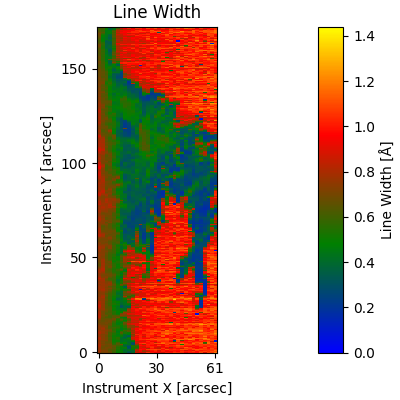
\includegraphics[width=0.5\linewidth]{./01Observations/figs/20180419/fwhmex.png} 
    \caption{\mgii~h Line Width map of raster 15 without the filter applied. The structure of the prominence is clearly distinguishable from the corona.}
    \label{fwhmex}
\end{figure}
\section{Concluding Remarks}

The prominence of 2018-04-19 is very dynamic with many flows and morphological changes through the IRIS observations. The line core shift from the quantile method demonstrates that the prominence is mainly dominated by redshifted flows relative to the solar disc. The large values of recovered asymmetry appear to be a by-product of spectral profiles with large line core shift interacting with the optical depth of the occulting plasma resulting in the absorption of parts of the line profile, exaggerating the asymmetry. This also affects the line core shift measurements, as the quantile method now overestimates the line core shift. The distribution of line core shifts found is different for \mgiihk{}, respectively.  This could be a result of \mgii~h generally having a smaller line width compared to \mgii~k or opacity effects. The prominence displayed a diverse range of line profile shapes, but was dominated by single peaked profiles due to the low column mass of the upper structure. Asymmetry is usually caused by the existence of multiple threads of different doppler velocity along the line of sight. If they are close enough in velocity, they will form what appears to a be a single asymmetric profile. This is another reason to only trust velocities where lower asymmetry is found. 

From these measurements that we can deduce directly from observations, very few conclusions can be drawn about the plasma conditions. This is where modelling is required to further our understanding of how these lines are formed, and what we can then further infer about our observations. 